% !TeX spellcheck = pl_PL
\newpage
\part{\huge \textbf{Analiza zadania}}
% --- Analiza zadania z dokumentu projektowego, poszerzoną o jasno wyszczególnione elementy, które podczas pracy zostały dodane/usunięte/uległy zmianie (z uzasadnieniem)
\indent \indent W tym rozdziale zostanie przedstawiona analiza zadania, jaka znalazła się w założeniach w dokumencie projektowym, poszerzona o informacje na temat faktycznej realizacji tego zadania.
\section{Podstawy teoretyczne problemu}
	\subsection{Przestrzeń fizyczna}
	\indent \indent W naszej grze w interakcję wchodzi ze sobą bardzo dużo elementów, począwszy od gracza, a na ostatnim z setki pocisków skończywszy. Bardzo ważne jest, aby ruchy i interakcje wszystkich elementów były ze sobą zsynchronizowane, a droga o długości 1 była tym samym dla każdego z nich. W tym celu zdecydowaliśmy się na wprowadzenie do gry przestrzeni fizycznej, w której będą zachodzić wybrane przez nas zjawiska fizyczne, potrzebne dla realizacji gry.

	\subsection{Ruch}
		\indent \indent Każdy obiekt, który może się poruszać i zmienić swoje położenia, posiada swoją prędkość. W naszej grze wyróżniliśmy 3 rodzaje ruchu:
	\subsubsection{Ruch jednostajny}
		\indent \indent W jednostce czasu ciało pokonuje jednakową drogę, a przebyta droga jest proporcjonalna do czasu.
		$$ v=\cfrac{s}{t}=const$$
		Gdzie $ v $ to prędkość, $ s $ - droga, a $ t $ to czas. W naszym obiekty poruszają się na ekranie, więc jednostką długości jest piksel.
	\subsubsection{Ruch jednostajnie przyspieszony}
		\indent \indent W jednostce czasu prędkość ciała ulega zwiększeniu o stałą wartość.
		$$ v(t)=v_0+a\cdot t $$
	\subsubsection{Ruch jednostajnie opóźniony}
		\indent \indent W jednostce czasu prędkość ciała ulega pomniejszeniu o stałą wartość.
		$$ v(t)=v_0-a\cdot t $$
	\subsubsection{{\large Komentarz}}
		\indent \indent Zrealizowaliśmy wszystkie 3 rodzaje ruchu. Każdy obiekt, który może się poruszać po planszy, posiada swoją stałą prędkość i przyspieszenie. Domyślnie obie wartości są równe zero - jeśli nie zostaną zdefiniowane podczas tworzenia obiektu, stoi on w miejscu. Można zdefiniować szybkość obiektu bez przyspieszenia (wówczas ma on stałą prędkość), ale nie można zrobić operacji odwrotnej.\\
		Nie definiowaliśmy żadnych innych rodzajów ruchu, te 3 w zupełności wystarczyły. Ich implementacja była prosta, a dzięki operatorom C++ jak += wygodniejsza niż wzory matematyczne.

\newpage
	\subsection{Tor pocisków}
		\indent \indent Jednym z podstawowych problemów w naszym zadaniu jest tor po jakim poruszają się pociski. Obiekty wrogów  poruszają się w prosty sposób, jednak zbiory pocisków mają układać się w skomplikowane wzory, tworzyć ze sobą specyficzny układ. W naszej grze chcemy zaimplementować pociski, które będą poruszać się m.in. po takich torach jak okrąg i elipsa.
	\subsubsection{Okrąg}
		\indent \indent Zdefiniowaliśmy ten rodzaj toru równaniem parametrycznym:
		$$
		\begin{cases}
		x=x_0+r\cdot \cos{\theta}\\
		y=y_0+r\cdot \sin{\theta}
		\end{cases}
		$$
		Gdzie punkt $ O(x_0, y_0) $ jest środkiem okręgu, $ r $ promieniem, a parametr $ \theta \in [0, 2\pi ) $.
	\subsubsection{Elipsa}
		\indent \indent Podobnie jak wyżej, elipsę zdefiniowaliśmy równaniem parametrycznym:
		$$
		\begin{cases}
		x=x_0+a\cdot \cos{\theta}\\
		y=y_0+b\cdot \sin{\theta}
		\end{cases}
		$$
		Gdzie punkt $ O(x_0, y_0) $ jest środkiem elipsy, $ a,\:b $ długościami półosi, a parametr $ \theta \in [0, 2\pi ) $.
	\subsubsection{Spirala}
		\indent \indent Będziemy wykorzystywać spirale z gatunku spiral Archimedesa. Tor takiej spirali jest zdefiniowany równaniem parametrycznym:
		$$
		\begin{cases}
		x=x_0+a\cdot \theta \cdot \cos{\theta}\\
		y=y_0+a\cdot \theta \cdot \sin{\theta}
		\end{cases}
		$$
		Gdzie punkt $ O(x_0, y_0) $ jest punktem centralnym spirali, $ a \in R $ , a parametr $ \theta \in [0, \inf ) $.
	\subsubsection{Spirala Fermata}
		\indent \indent Typ spirali zdefiniowany równaniem parametrycznym:
		$$
		\begin{cases}
		x=x_0+a\cdot \sqrt{\theta} \cdot \cos{\theta}\\
		y=y_0+a\cdot \sqrt{\theta} \cdot \sin{\theta}
		\end{cases}
		$$
		Gdzie punkt $ O(x_0, y_0) $ jest punktem centralnym spirali, $ a \in R $, a parametr $ \theta \in [-inf, \inf ) $.
	\subsubsection{Spirala hiperboliczna}
		\indent \indent Typ spirali zdefiniowany równaniem parametrycznym:
		$$
		\begin{cases}
		x=x_0+ae^{b\theta} \cdot \cos{\theta}\\
		y=y_0+ae^{b\theta} \cdot \sin{\theta}
		\end{cases}
		$$
		Gdzie punkt $ O(x_0, y_0) $ jest punktem centralnym spirali, $ a,b \in R $, a parametr $ \theta \in [0, \inf ) $.
	\subsubsection{{\large Komentarz}}
		\indent \indent Zaimplementowaliśmy wszystkie rodzaje w/w torów. Wszystkie charakteryzują się tym, że można je zdefiniować parametrycznie wykorzystując kilka zmiennych. Dzięki temu wygodnie mogliśmy utworzyć klasę bazową, zawierającą całą wspólną funkcjonalność, a pochodne jedynie zmieniały uzyskiwaną drogę. Wszystkie drogi można było generować na pomocą fabryki. Nie utworzyliśmy dodatkowych klas.\\
		\indent Podczas testów jedyną niepraktyczną drogą okazała się \textbf{spirala hiperboliczna}. Zbyt szybko rośnie, przez co pociski bardzo szybko wylatywały poza planszę nie stanowiąc żadnego zagrożenia. Żeby móc ją zastosować, należało tej spirali przydzielać bardzo małe parametry, bliskie zeru.

\newpage
\section{Wykorzystywane zagadnienia grafiki komputerowej}
	\subsection{Przekształcenia afiniczne}
		\indent \indent Postanowiliśmy wykorzystać poznane na laboratorium przekształcenia afiniczne. Wszystkie ruchome obiekty w naszej grze, które zmieniają dynamicznie swoją pozycję w przestrzeni dwuwymiarowej, korzystają z trzech wybranych przekształceń:
		\subsubsection{Translacja}
			\indent \indent Przesunięcie punktu $ P=(x, y) $ o wektor $ d=[d_x, d_y] $, w wyniku którego powstaje obraz\\ $ P=(x', y') $, gdzie:
			$$
			\begin{cases}
			x'=x+d_x\\
			y'=y+d_y
			\end{cases}
			$$
		\subsubsection{Skalowanie}
			\indent \indent W naszym programie wszystkie przekształcenia skalowania będą zachowywać proporcje, więc zdefiniować je jako: przesunięcie punktu $ P=(x, y) $ o współczynnik skalowania $ s $, w wyniku którego powstaje obraz\\ $ P=(x', y') $, gdzie:
			$$
			\begin{cases}
			x'=s\cdot x\\
			y'=s\cdot y
			\end{cases}
			$$
		\subsubsection{Obrót}
			\indent \indent Obrót punktu $ P=(x, y) $ wokół początku układu $ O=(0, 0) $ da nam obraz $ P=(x', y') $, gdzie:
			$$
			\begin{cases}
			x'=x\cos(x)-y\sin(x)\\
			y'=x\sin(x)+y\cos(x)
			\end{cases}
			$$
		\subsubsection{{\large Komentarz}}
			\indent \indent Przekształcenia afiniczne okazały się podstawą dla ruchu i przekształceń wszystkich obiektów w grze. Utworzyliśmy interfejs ITransformable, który wymusza zastosowanie tych trzech przekształceń. W naszej grze implementuje go GameObject, a co za tym idzie, również wszystkie obiekty, które są elementami planszy, m.in. Player, Bullet, Enemy i Bonus.\\
			\indent Interfejs ten implementują także klasy "niewidoczne" - Hitbox oraz Trajectory.
			\begin{itemize}
				\item Hitbox jest polem uderzeń dla każdego GameObjectu i podstawą do wykrywania kolizji, zatem jeśli nadrzędny GameObject zmianie miejsce lub rozmiar, Hitbox również musi to zrobić.
				\item Tor po którym poruszają się obiekty również może zmieniać swój kształt. Przykładowo, jeśli tor elipsy zwiększy swoją skalę dwukrotnie, wszystkie elementy, które się po nim poruszają, będą poruszać się po większym polu i przebywać swoją drogę 4 razy dłużej.
			\end{itemize}
			\indent Zastosowanie przekształceń afinicznych staraliśmy się upraszczać do jak najmniejszej liczby obliczeń. Jeżeli dany typ obiektu mógł skutecznie wykonać operację szybciej, korzystając z prostych obliczeń, to przeciążał odpowiednią metodę. Jeżeli nie mógł tego zrobić, to korzystał z ogólniejszej metody nadrzędnej.
\newpage
\subsection{Krzywe i powierzchnie parametryczne}
	\indent \indent W naszym projekcie pojawią się krzywe parametryczne. Będą spełniać rolę toru pocisków. W celu opisania krzywej na przestrzeni $ n $-wymiarowej są potrzebne $ n $ funkcji, które opisują współrzędne punktów tej krzywej. My wykorzystamy z wielomianów 3 stopnia, ponieważ są wystarczająca elastyczne jeśli chodzi o zmianę kształtu krzywej i nie powodują wykonywania dużej ilości dodatkowych obliczeń.
	Wielomian opisujący segment krzywej:
	$$ Q(t)=[\:x(t)\:y(t)\:z(t)\:]^T  \:\:\:\:\:\: 0 \leq t \leq 1 $$
	Gdzie:
	\begin{itemize}
		\item $ x(t)= a_x t^3+b_x t^2+c_x t+d_x $
		\item $ y(t)= a_y t^3+b_y t^2+c_y t+d_y $
		\item $ z(t)= a_z t^3+b_z t^2+c_z t+d_z $
	\end{itemize}
	
	\subsubsection{Krzywe Beziera}
		\indent \indent Fragment krzywej Beziera opisywany jest przez dwa punkty końcowe $ P_0 $ i $ P_3 $ (interpolacja) i dwa punkty pośrednie $ P_1 $ i $ P_2 $ (aproksymacja), które decydują o postaci wektorów w punktach końcowych.\\Krzywą Beziera trzeciego stopnia definiuje równanie wielomianowe:
		$$ Q(t)=(1-t)^3\cdot P_0+3t\cdot(1-t)^2\cdot P_1+3t^2(1-t)\cdot P_2+t^3\cdot P_3 $$
		
	\subsubsection{{\large Komentarz}}
		\indent \indent W naszym projekcie zastosowaliśmy krzywe Beziera zgodnie z zaprezentowanymi wzorami. W tym celu zdefiniowaliśmy osobną rodzinę klas, które definiują trasę obiektu na podstawie wskazanych przez projektanta punktów. Implementacja nie była trudna, należało jedynie zdefiniować punkty i wykonać obliczenia. Większym wyzwaniem było wczytywanie punktów z pliku i przekazanie ich do klasy.\\\\
		\indent Ponieważ krzywą Beziera napisaliśmy najpóźnmiej ze wszystkich rodzajów torów, implementację musieliśmy dostosować do już istniejących realiów - jako reprezentację ruchu po torze wybraliśmy obliczanie położenia na podstawie przebytego dystansu. Obiekty, które mogą się poruszać, posiadają swoją prędkość z którą pokonują drogę. Aby obiekty, które poruszają po się liniach, elipsach i spiralach, robiły to zgodnie (żeby np. przy linii nie brać długości, a przy elipsie kąta), znają one wyłącznie swój dystans. Obiekt wie, że w czasie 1 sekundy pokonał \emph{n} pikseli drogi, z kolei to obiekt drogi wie, że to połowa odcinka lub ćwiartka obwodu lub jedno zatoczenie spirali.\\\\
		\indent Problem pojawił się właśnie podczas późniejszej implementacji krzywej Beziera. Aby algorytm wyznaczania dystansu mógł działać, należy po prostu znać długość trasy, by móc ją odwzorować na planszy. Jednak obliczanie długości dla krzywej Beziera wymaga ogromnej liczby obliczeń. Dla 3 punktów istnieje ogromny wzór, z kolei na 4 punktów należy ją wyznaczyć metodą aproksymacji. Zastosowane rozwiązanie umożliwiło nam budowanie krzywych Beziera na maksymalnie 4 punktach.\\\\
		\indent Wybrane rozwiązanie co prawda umożliwiło nam spełnienie założeń (krzywa Beziera na 4 punktach), ale uniemożliwiło wyjście poza nie.
		

\newpage
\subsection{Wykrywanie kolizji}
	\indent \indent Jako kolejne zagadnienie wykorzystaliśmy wykrywanie kolizji. Jest ono potrzebne ze względu na zderzenia pocisków z obiektami i przeciwnikami. Naszym zadaniem będzie wykrycie, że kolizja miała miejsce i odpowiednia reakcja na tę sytuację (utrata życia, animacja zderzenia itd.).\\\\
	\indent Z dwóch rodzajów kolizji, statycznych i dynamicznych, zdecydowaliśmy się na realizację tych pierwszych. Są prostsze do realizacji, wymagają mniej obliczeń i szerzej omówione w ramach laboratorium. Aby uniknąć potencjalnych problemów związanych ze sprawdzaniem stanu klatka po klatce będziemy ograniczać prędkość pocisków tak, by nie występowało omijanie kolizji.\\\\
	\indent W celu optymalizacji tego procesu będziemy stosować zmodyfikowaną metodę sfery otaczającej - zamiast otaczać cały model kulą, będzie się ona znajdować w jego wnętrzu na scenie 2D jako tzw. \emph{Hitbox}. Podobnie jak przy sferze otaczającej, jego środek równy środku sprajta, lecz jego promień będzie odpowiednio mniejszy. Każdy element gry, z którym gracz może wejść w kontakt, będzie posiadał swój Hitbox. Elementy takie jak tło czy pasek życia nie będą go miało i pozostaną tylko rysunkami.\\
	W celu testowania kolizji będzie stosować prostą metodę \emph{circle - circle}.
	\begin{center}
		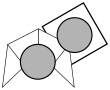
\includegraphics[width=0.2\textwidth]{./images/kolizja}
	\end{center}
	Ilustracja: jak widać, chociaż oba sprajty na siebie nie nachodzą, do kolizji nie dochodzi gdyż oba Hitboxy są od siebie oddalone.
	\subsection{{\Large Komentarz}}
		\indent \indent Wykrywanie kolizji było jednym z największych wyzwań w całym projekcie. Pozornie temat wydaje się bardzo prosty, jednak prawidłowa implementacja i oszczędność obliczeń stanowiły nie lada trud.\\\\
		\indent W naszej grze na planszy często znajduje się wielka liczba pocisków, zarówno wrogich jak i naszych, oraz samych wrogów. Dla każdej aktualizacji sceny gry należy sprawdzić, czy:
		\begin{itemize}
			\item Gracz zderzył się z którymkolwiek z pocisków
			\item Gracz otarł się o którykolwiek z pocisków
			\item Wróg zderzył się z którymkolwiek z pocisków gracza lub jego bombą
			\item Gracz zderzył się z którymś z bonusów
		\end{itemize}
		Co czasem mogło doprowadzić do tysięcy testów na klatkę. Szybko okazało się, że pomimo niewielkiego rozmiaru naszej gry, rzędu 300 KB w wersji Release, potrafiła ona zająć ponad 100 MB RAMu. Prowizoryczne rozwiązania były nieefektywne, więc zaczęliśmy szukać skuteczniejszych.
	\subsubsection{Okrąg czy elipsa?}
		\indent \indent W trakcie naszej pracy nad programem początkowo wykorzystywaliśmy okrąg do sprawdzania kolizji. Wysokość i szerokość wszystkich sprajtów była w przybliżeniu równa, więc punkty środkowe okręgu i sprajta były równe, a promieniem był krótszy z boków. Jednak po czasie pojawiły się kształty (np. bomba), dla których obsługa kolizji poprzez okrąg wyglądałaby nieatrakcyjnie. Wówczas postanowiliśmy wykorzystać elipsę. Okrąg jest jedynie specjalnym przypadkiem elipsy o równych półosiach. Gdy obiekt miał mieć hitbox w kształcie elipsy, dłuższy bok definiował długość jednej półosi, a krótszy drugiej.
		\newpage
		\indent Rozwiązanie to okazało się bardzo mało efektywne - do wykrywania kolizji potrzebny były dodatkowy parametr, kąt pomiędzy obiektami. Dla jednego testu należało obliczyć ten kąt, następnie obliczyć długość promienia elipsy dla tego kąta u obu obiektów i dopiero wtedy była znane zajście kolizji. Dla hitboxów o równych osiach powodowało to mnóstwo niepotrzebnych obliczeń. Nawet pominięcie ich w przypadku równych półosi wymagało obliczania i przekazania kąta, który dla każdej elipsy był niezbędny.\\\\
		W takiej sytuacji mieliśmy dwie możliwości:
		\begin{enumerate}
			\item \textit{Zmiana elipsy wieloma okręgami} - eliminuje wykorzystanie elipsy, jednak dla każdego obiektu jest potrzebne zdefiniowanie ile okręgów potrzebuje, w którym miejscu i o jakiej wielkości, tak, by dopasować je do kształtu sprajta. Projektowanie ciała okręgów byłoby niezwykle niewygodne bez wsparcia designerskiego, którego nasza gra nie miała. 
			\item \textit{Osobne klasy dla okręgu i elipsy} - okręgu potrzebowałyby jak najmniejszej liczby danych i obliczeń, a elipsa pozostałaby obsługiwana. Wadą jest naruszenie zasad polimorfizmu - przy każdym teście okręgi nie potrzebują kąta między obiektami, więc przekazywanie ich jest zbędne i prowadzi do niepotrzebnych operacji.
		\end{enumerate}
	\subsubsection{Zastrzyk zależności}
		\indent \indent Rozwiązaniem problemu opisanego w powyższym rozdziale okazał się wzorzec projektowy, zastrzyk zależności (\emph{dependency injection}). Realizujemy go w ten sposób, że przy każdym teście kolizji, do jednego hitboxa wstrzykujemy drugi - pierwszy zna swoje metody działania, rzutuje drugi na odpowiedni typ i sprawdza kolizję zwracając true lub false.\\\\
		\indent Rozwiązanie jest skuteczne, ponieważ jeżeli w teście kolizji znajduje się elipsa, to pobiera one dane jakiej jej potrzeba. Jeżeli nie, test wykonywany jest najmniejszym możliwym kosztem. Sprawdzaniem, z którym typem hitboxa mamy do czynienia zajmuje się mechanizm RTTI.\\\\
		\indent Rozwiązanie to również znacznie przyspieszyło obliczenia, ponieważ dzięki temu została zmniejszona liczba wywołań funkcji oraz zakapsułkowała całe sprawdzenie kolizji do jednej metody.\\\\
		\indent Rozwiązanie to zostało zainspirowane sprawdzaniem kolizji, jakie wykonuje silnik Unity-chan.

\section{Wykorzystywane biblioteki i narzędzia programistyczne}
	\subsection{DirectX 9}
		\indent \indent Jako narzędzie do budowania obiektów graficznych zdecydowaliśmy się na DirectX w wersji 9. Jako alternatywne rozwiązanie rozważaliśmy DirectX 11, jednak nasza gra będzie budowana na scenie 2D, a DirectX 9 oferuje wygodniejsze narzędzia - wciąż operuje na takich klasach jak Sprite lub Texture, które są lepsze dla naszej gry. DirectX 11 wszystkie te klasy zastępuje interfejsem IResource, który wymaga odpowiedniej konwersji (większe nastawienie na grafikę trójwymiarową). By móc wykorzystać DirectX 11 do pracy na zwykłych sprajtach, wymagane byłyby dodatkowe zestawy narzędzi, jak np. DirectX Tool Kit.\\
		Jako konkurencyjne rozwiązanie dla samego DirectXa rozważaliśmy OpenGL, jednak nasz program będzie zorientowany obiektowo, a DirectX daje lepsze możliwości enkapsulacji.\\
		Ponadto, dzięki DirectXowi wygodniejsze jest pracowanie m.in. z przekształceniami afinicznymi modeli 3D.
	
	\subsection{Microsoft Visual Studio 2012}
		\indent \indent Wybraliśmy to środowisko ze względu na przyjazny interfejs, który nawet w najtrudniejszych sytuacjach potrafi okazać się bardzo pomocny. Pracujemy na nim od dłuższego czasu co ułatwi nam szybki dostęp do potrzebnych narzędzi. Etap debugowania posiada wiele możliwości kontroli naszego programu, co na pewno pozwoli uniknąć kilku czasochłonnych błędów. Ponieważ czasami pojawiają się problemy w kompilacji związane z różnymi wersjami VS, wspólnie wybraliśmy jedną wersję środowiska w celu usunięcia tych przeszkód.
	
	\newpage
	\subsection{Enterprise Architect}
		\indent \indent Jako narzędzie do zaprojektowania gry w modelu zorientowanym obiektowo wybraliśmy Enterprise Architect. Głównym powodem była nasza znajomość języka UML, którego uczymy się na studiach od ponad roku, a także doświadczenie z tym środowiskiem. Zdecydowaną zaletą wcześniejszego zaprojektowania aplikacji w tym środowisku jest wygoda obsługi, łatwość tworzenia diagramów oraz możliwość generacji kodu. Samo zdecydowanie się na wcześniejsze utworzenie diagramów UML umożliwi nam lepszą kontrolę nad pracą oraz zapewnienie wszystkich potrzebnych możliwości naszej aplikacji.
	
	\subsection{Inkscape \& Photoshop}
	Naszymi narzędziami graficznymi zostały:
	\begin{itemize}
		\item \textbf{Inkscape}: bardzo wydajny i zaawansowany program do grafiki wektorowej. Posiada ogromne możliwości w tworzeniu prostych i złożonych figur geometrycznych, ma bardzo dużą gamę tekstur oraz dzięki dobrym filtrom umożliwia tworzenie ciekawych efektów niewielkim kosztem. Dzięki operowaniu na grafice wektorowej umożliwia pracę na figurach i ich konwersję do popularnych formatów obrazków (JPEG, PNG) w wybranej rozdzielczości bez utraty jakości. Ponadto Inkscape posiada wsparcie dla grafiki 3D.
		\item \textbf{Adobe Photoshop}: drugi, również bardzo dobry program do tworzenia zaawansowanej grafiki 2D. Operuje na pikselach, lecz posiada klasyczny zestaw narzędzi (np. pędzel, gumka), które umożliwiają bardziej intuicyjne tworzenie grafiki. Dzięki wygodnej obsłudze warstw, licznym filtrom i narzędziom w szczególności umożliwia dobrą edycję rysunków.
	\end{itemize}
	
	\subsection{{\Large Komentarz}}
		\indent \indent W czasie naszej pracy nad programem korzystaliśmy dokładnie z tych narzędzi. Cała praca odbywała się w środowisku Visual Studio, które później wzbogaciliśmy m.in. o wtyczkę do generowania dokumentacji, GhostDoc. Kontrola wersji odbywała się poprzez GitHub i tam znajduje się repo wraz z całą historią. Wadą GitHuba okazało się wadliwe działanie konfiguracji .ignore, przez co nie mogliśmy automatycznie niecommitować śmieci powstałych z kompilacji i innych niechcianych rzeczy na repozytorium,. Często zdarzało się wrzucić coś niechcianego na serwer co skutkowało koniecznością modyfikowania historii repozytorium.\\\\
		\indent Prawie wszystkie sprajty zostały narysowane przez nas w programach Photoshop oraz Inkscape, a projekt UML program został stworzony w Enterprise Architect. Nie korzystaliśmy z innych dodatkowych narzędzi.
\newpage
\section{Algorytmy, struktury danych, ograniczenia specyfikacji}
	\subsection{Algorytm De Casteljau}
		\indent \indent W naszym programie konieczne okazało się zastosowanie tylko jednego algorytmu, do tworzenia krzywych Beziera. Wybraliśmy algorytm De Casteljau, który jest prosty w zrozumieniu i implementacji, ponadto był omawiany na wykładach profesora Wojciechowskiego.\\\\
		\indent \emph{Zasada działania}: krzywa sześcienna przedstawiona jest jako 4 punkty kontrolne. Algorytm dzieli odcinki $ P_0 P_1 $, $ P_1 P_2 $, $ P_2 P_3 $ w proporcji $ t\: : \: 1-t $, gdzie $ t \in [0, 1] $. Operację tę należy powtarzać aż do momentu otrzymania pojedynczego punktu $ P(t) $. Uzyskany punkt leży na krzywej Beziera i dzieli ją na dwie części o punktach kontrolnych $ P_0 P_0^1 P_0^2 P(t) $ i $ P(t) P_1^2 P_2^1 P_3 $.
		\\
		Pseudokod:
		\begin{lstlisting}[language=Ada, frame=single, autogobble=true, commentstyle=\ttfamily\itshape\color{gray}, frameround=ffff,rulecolor=\color{black}, tabsize=4]
			-- P[n] - tablica n punktow kontrolnych
			-- t - wspolczynnik z przedzialu od 0 do 1
			function deCasteljau(P[n], t)
			begin
				for  i:=0 to n do
					Q[i] := P[i];
					for k:=1 to n-k do
						Q[i] := (1-t) * Q[i] + t * Q[i+1];
					end for;
				end for;
				return Q[0]; -- punkt na krzywej Q(t)
			end.
		\end{lstlisting}
		\subsubsection{{\large Komentarz}}
			\indent \indent Algorytm został zastosowany w klasie zajmującej się realizacją toru na krzywej Beziera. Klasa oblicza długość krzywej Beziera, normalizuje ją do wartości jeden, a następnie pobiera dystans jaki przebiegł obiekt, sprawdza jaka to jest część krzywej Beziera i zwraca jego pozycję na planszy.\\
			\indent Złożoność obliczeniowa algorytmu nie jest najkorzystniejsza, ale przy ciągłym obliczaniu punktów na kilku krzywych Beziera jednocześnie, na współczesnym komputerze domowym nie wpływa to na jakość rozgrywki.
			